\section{Database}
\label{sec:database}
Il database dopo la fase di ristrutturazione risulta essere costituito da 6 entità principali:
\begin{figure}[H]
    \centering
    \makebox[\textwidth][c]{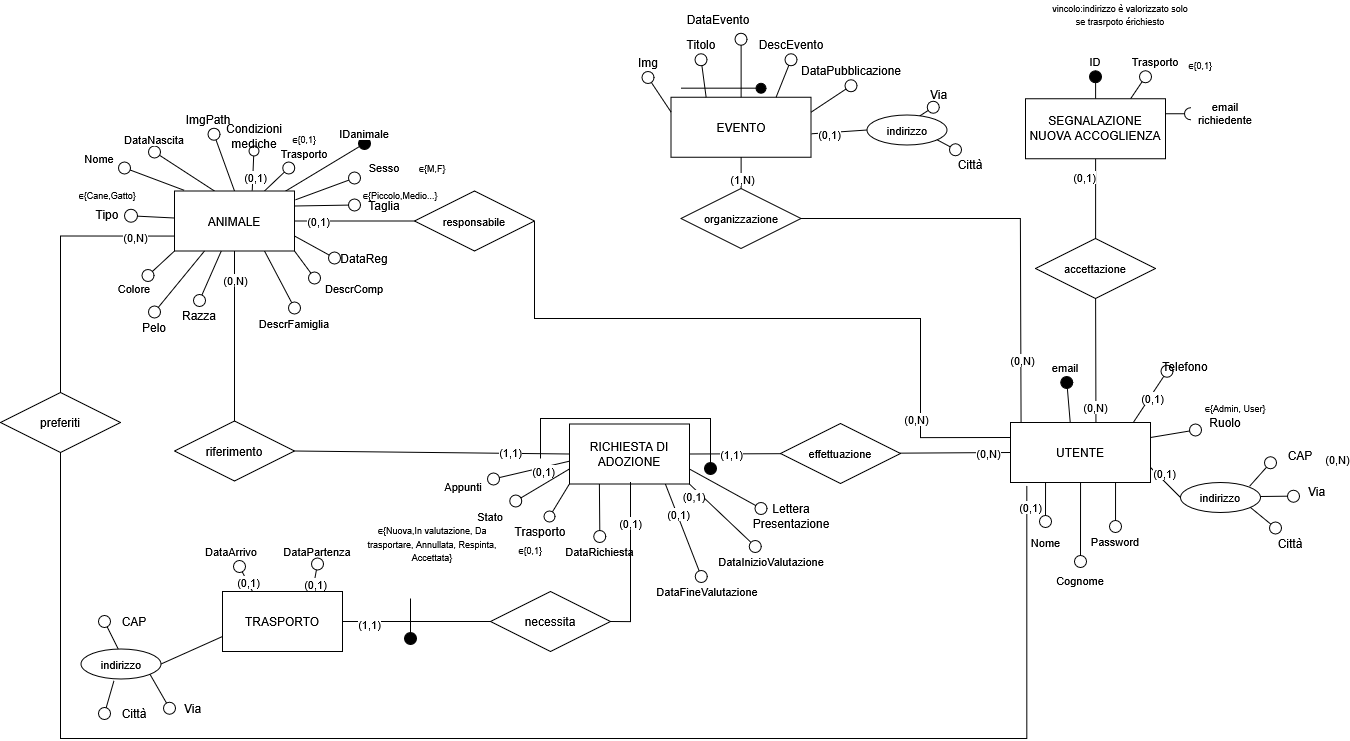
\includegraphics[width=1.35\textwidth]{assets/schema-er.png}}
    \caption{Schema ER del database}
    \label{fig:schema-er-database}
\end{figure}

Alcune considerazioni sul database:
\begin{itemize}
    \item Per questione di semplicità, utente normale e admin sono stati unificati in un'unica entità \texttt{Utente}, differenziata da un attributo \texttt{Ruolo}.
    \item Abbiamo deciso, in fase di implementazione in SQL, di non esprimere i vincoli interrelazionali poichè non studiati nel nostro corso di studi. Questi vincoli sono stati gestiti a livello di logica applicativa (php). Alcuni vincoli interrelazionali sono:
    \begin{itemize}
        \item Un trasporto è associato ad una richiesta solo se la richiesta è in "In trasporto" e il trasporto è stato richiesto (Attributo Trasporto =1)
        \item I preferiti esistono solo per utenti di ruolo \texttt{User}
        \item Una richiesta di adozione non fa mai riferimento ad un animale già adottato.
        \item Abbiamo deciso di non inserire elementi aggiuntivi sugli animali per distinguere la lingua della razza o del nome, poiché non ci sembrava giusto modellare il database alle necessità del web e inoltre risultava eccessivo dal nostro punto di vista. Perciò non è presente l'attributo lang nelle razze non italiane o nei nomi degli animali.
    \end{itemize}
\end{itemize}